\section{Literature Review}

The review will be structured as follows. The first section will explore what is meant by data quality in the context of wireless sensor networks (WSN) and examine the established taxonomies for quantifying data quality. The second section will investigate common methodologies used to assess data quality in WSN. The third section, which will be the main focus of the forthcoming research, will investigate methods for detecting and monitoring data quality in real-time. The fourth section will briefly investigate the methods used to manage and improve data quality such as automated methods for missing data-imputation and denoising. The fifth section, also brief, will explore the methods used to improve the design of WSN architecture so as to improve future data quality from the source. The final section will explore the challenges and future directions in building quality-aware platforms for smart cities.

\begin{itemize}
    \setlength{\itemindent}{3cm}
    \raggedright
    \item[\ref{ssec:data_quality_dimensions}] \textit{Data Quality Dimensions and Metrics}
    \item[\ref{ssec:data_quality_assessment}] \textit{Data Quality Assessment}
    \item[\ref{ssec:data_quality_detection}] \textit{Data Quality Detection and Monitoring}
    \item[\ref{ssec:data_quality_management}] \textit{Data Quality Management and Improvement}
    \item[\ref{ssec:data_quality_prediction}] \textit{Data Quality Prediction and Proactive Approaches}
    \item[\ref{ssec:challenges_and_future_directions}] \textit{Challenges and Future Directions}
\end{itemize}

\subsection{Data Quality Dimensions and Metrics} \label{ssec:data_quality_dimensions}

Defining data quality can be challenging due to its multifaceted nature and the number of ways it can be assessed. Establishing a clear understanding of what constitutes data quality is crucial, particularly in the context of sensed pedestrian data. Identifying the most relevant aspects of data quality for pedestrian counting WSNs enables a targeted approach to developing quality-aware systems.

\subsubsection{Data Quality Taxonomy}

DQ taxonomies have developed significantly over the last few decades as technology has developed and the age of ‘big data’ and IoT has emerged. Although it is difficult to identify a single “seminal” paper on DQ, one of the most influential and widely cited papers on DQ dimensions is \cite{wangAccuracyWhatData1996}. The authors describe DQ as ‘data that are fit for use by data consumers’. Their taxonomy presented in Figure \ref{fig:seminal_dq_taxonomy} describes four main categories of DQ dimensions: intrinsic, contextual, representational, accessibility.

    {\color{secondary-text-color} \textit{NOTE: Taxonomies, as described by the methodology produced by \cite{nickersonMethodTaxonomyDevelopment2013}, consist of a set of dimensions that in turn consist of mutually exclusive characteristics.}}

\begin{figure}[h]
    \centering
    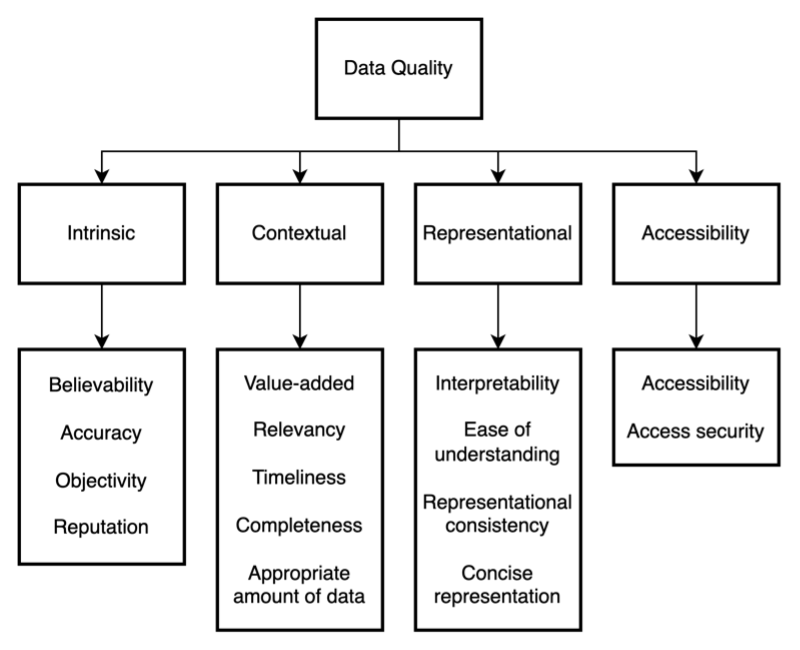
\includegraphics[]{figures/literature_review/seminal_dq_taxonomy.png}
    \caption{‘Seminal’ DQ taxonomy from \cite{wangAccuracyWhatData1996}}
    \label{fig:seminal_dq_taxonomy}
\end{figure}

\subsubsection{Internet of Things Data Quality Taxonomy}
IoT data is highly structured (follows a schema) and can therefore use a narrower taxonomy with more precise definitions of dimensions. \cite{karkouchDataQualityInternet2016} point out that many DQ dimensions have inconsistent definitions depending on the source. For example timeliness can (among other definitions) be defined as “currency” (when the data was last updated) \citep{dasuExploratoryDataMining2003}, or the average age of data in a source \citep{naumannQualitydrivenQueryAnswering2002}. The categories of intrinsic, contextual, representational and accessibility have remained consistent throughout taxonomies since \cite{wangAccuracyWhatData1996}. A simplified DQ taxonomy for IoT is presented in Figure \ref{fig:iot_dq_taxonomy}.

\begin{figure}[h]
    \centering
    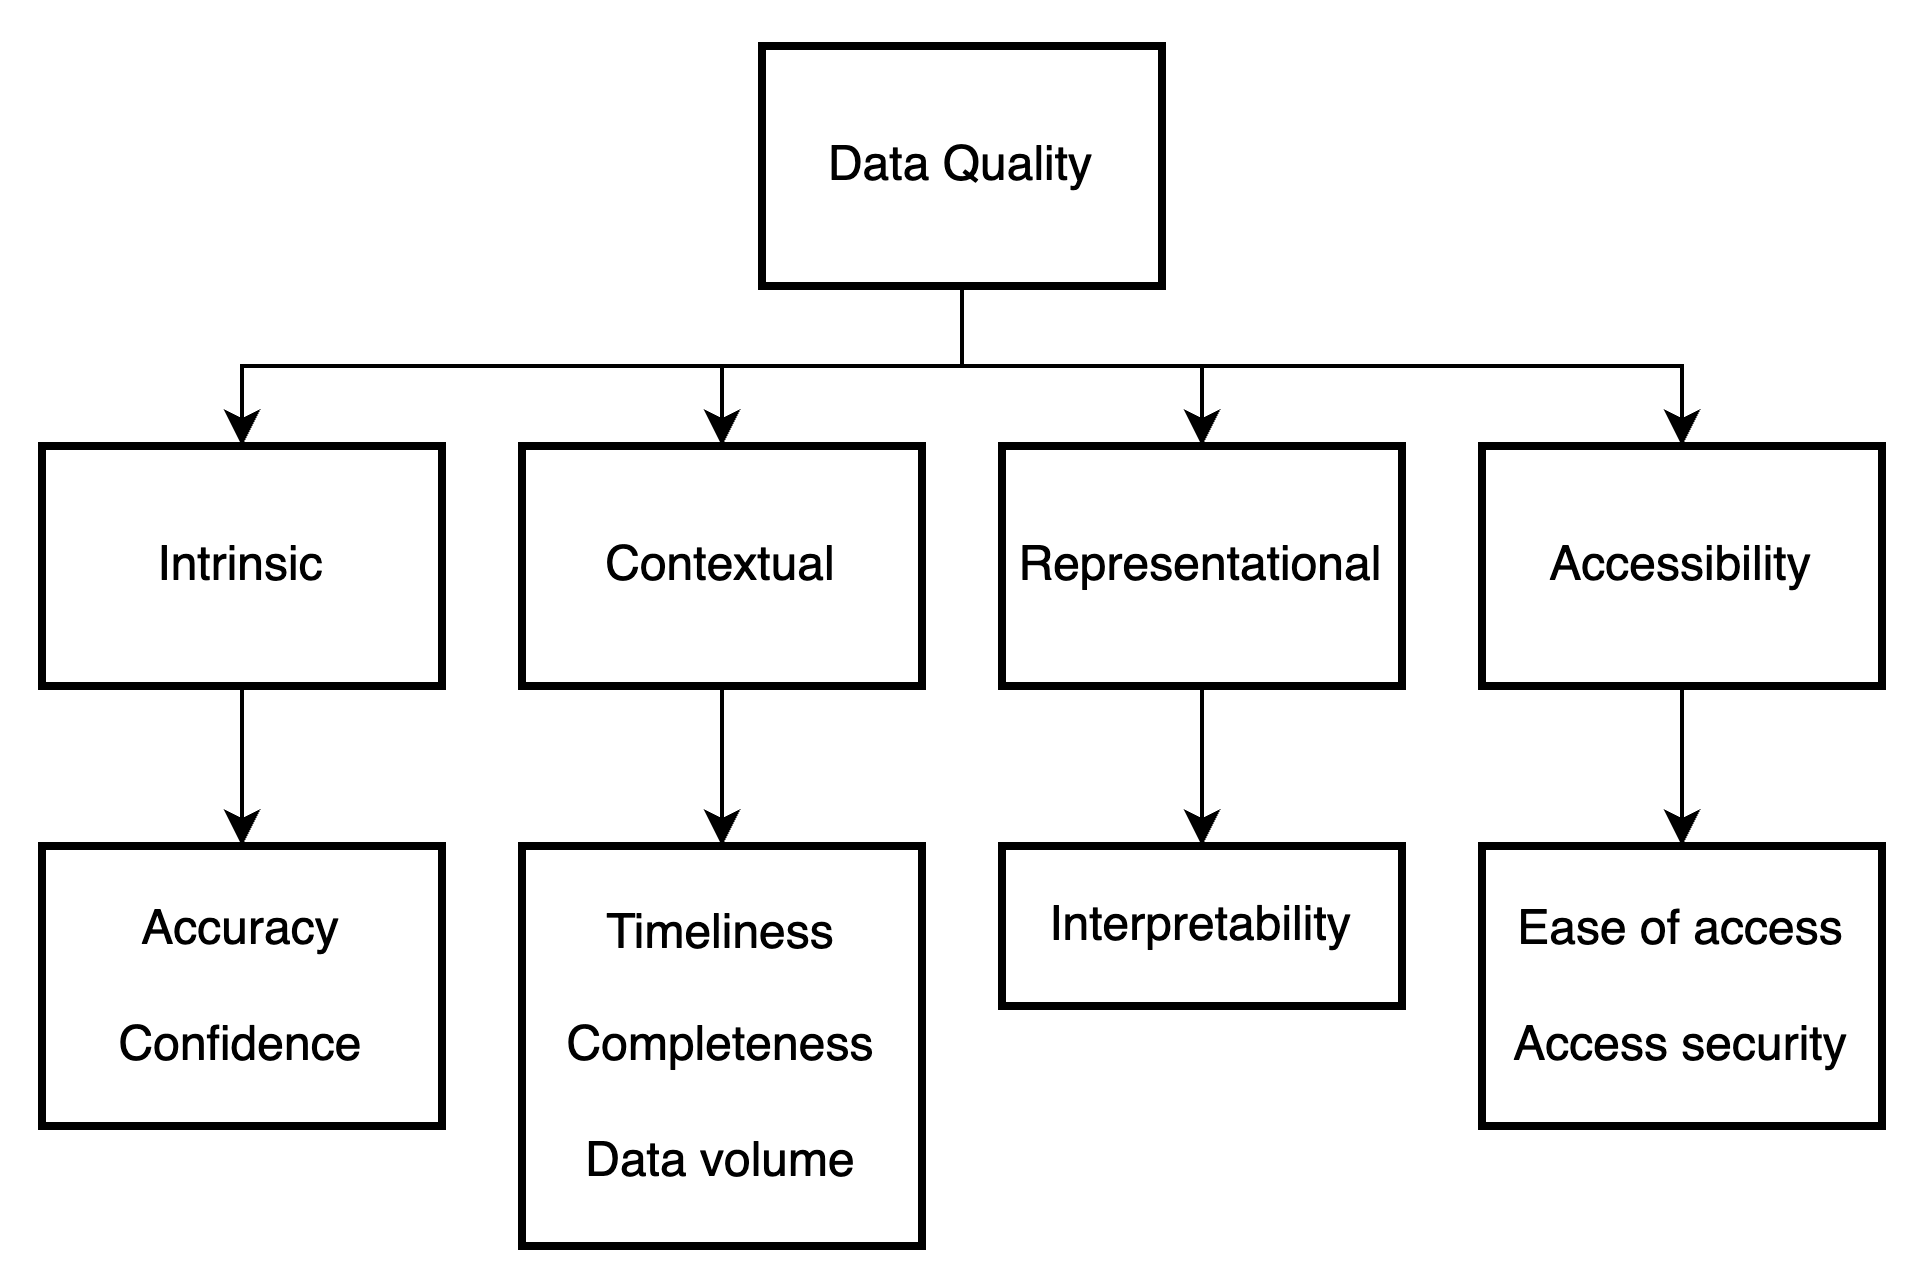
\includegraphics[scale=0.15]{figures/literature_review/iot_dq_taxonomy.png}
    \caption{IoT DQ taxonomy based on \cite{karkouchDataQualityInternet2016}}
    \label{fig:iot_dq_taxonomy}
\end{figure}

Data quality taxonomies form a hierarchy---the top level in figure \ref{fig:taxonomy_subsets} encompass all data quality issues (DQ), internet-of-things data quality (IoT DQ) issues form a subset \citep{batiniDataInformationQuality2016} followed by wireless sensor network data quality issues (WSN DQ). Existing taxonomies for WSN DQ are most relevant to this research and will be used as a foundation.

However, it is important to recognise that some DQ issues outlined in these taxonomies may not be applicable to this specific research, while other issues not covered in the taxonomies may arise, particularly those related to the performance of object detection algorithms (OD DQ). Whilst there are no taxonomies focussed on data from object detecting WSN, there are taxonomies focussed on deep-learning based object counting methodologies, which to some extent, cover data quality issues \citep{heinrichEverythingCountsTaxonomy2019}.

\begin{figure}[h]
    \centering
    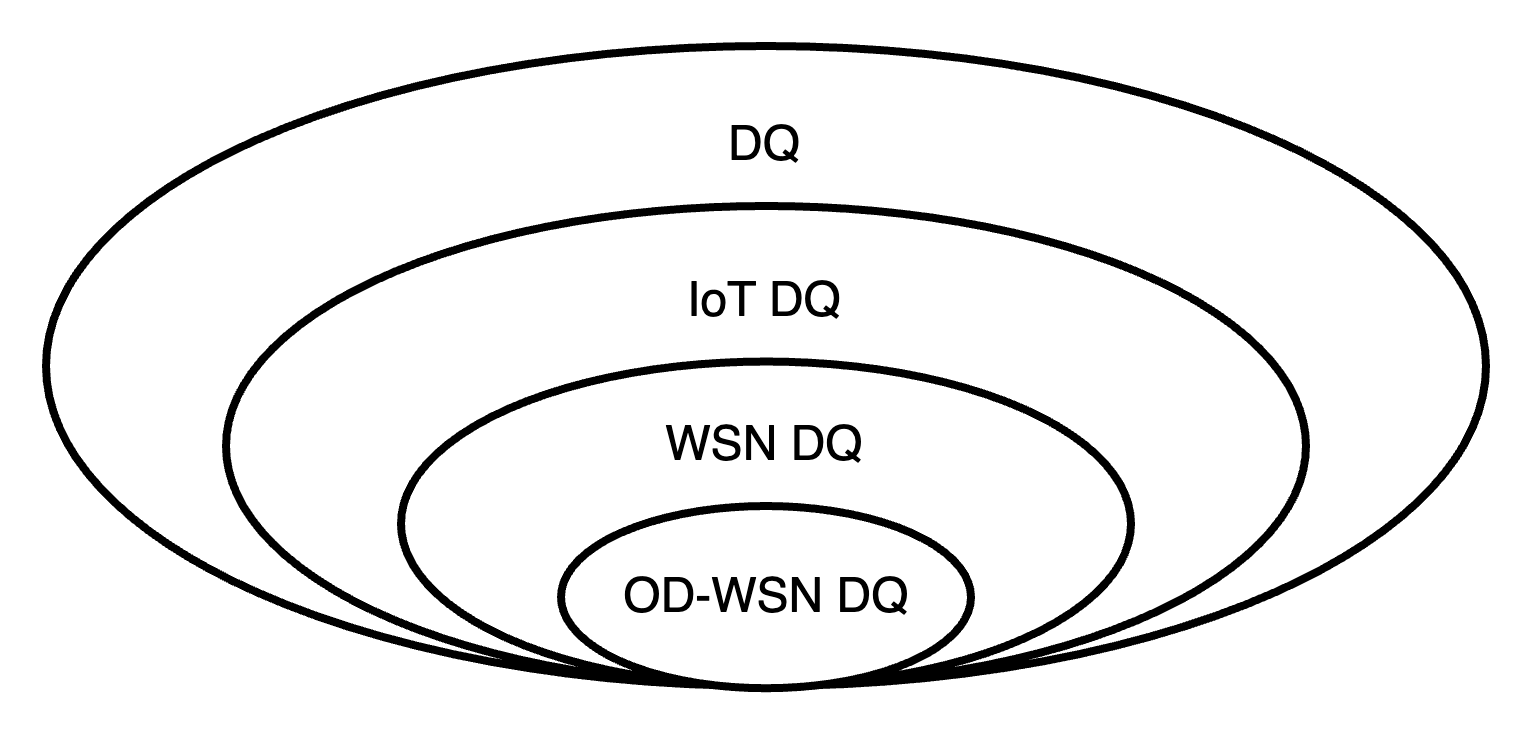
\includegraphics[scale=0.15]{figures/literature_review/taxonomy_subsets.png}
    \caption{Subsets of taxonomies for data quality}
    \label{fig:taxonomy_subsets}
\end{figure}

\subsubsection{Adopted Dimensions for Data Quality}
\cite{mansouriIoTDataQuality2023} provides a reliable and recent review of IoT data quality literature. Whilst there are limited significant changes to the dimensions proposed by \cite{karkouchDataQualityInternet2016}, the authors map key issues to the core dimensions from the \cite{karkouchDataQualityInternet2016} framework, whilst highlighting how these issues arise from specific set of problems. The authors highlight the relationship between dimensions, problems and issues---how multiple issues can impact a single dimension and how a single problem can result in multiple data quality issues. Table \ref{table:dq_dimensions} shows the key WSN-DQ dimensions identified by the authors that will be adopted for this research:

% tables/literature_review/dq_dimensions.tex
\begin{table}[H]
    \centering
    \scriptsize % Reduce font size
    \begin{tabular}{|R{2cm}|R{2cm}|R{5cm}|R{5cm}|}
        \hline
        \textbf{Data Quality Dimension} & \textbf{Sub-Dimension} & \textbf{Description}                                                          & \textbf{Factors to consider}                                                                                          \\ \hline
        Accuracy                        & Preciseness            & How close the measured values are to the true values.                         & Measured values, sensor precision, measurement units, and granularity.                                                \\ \hline
        Accuracy                        & Certainty              & The confidence or probability that a measured value is true.                  & Sensor calibration, environmental conditions, and measurement techniques, and statistical confidence intervals.       \\ \hline
        Accuracy                        & Confidence             & Represents the reliability and credibility of the data source.                & Sensor provider's reputation, sensor's conformance to specifications, certification, and independent testing results. \\ \hline
        Timeliness                      & Freshness              & The degree to which data is recent and not obsolete.                          & Time of last reading, data expiration policies, and data lifecycle management.                                        \\ \hline
        Timeliness                      & Frequency              & How often the data is collected or updated.                                   & Expected measurement frequency, data collection intervals, and synchronisation between data sources.                  \\ \hline
        Completeness                    & Availability           & Percentage of data values actually recorded compared to the expected number.  & Existing data, historic expected measurement frequency, data gaps, and reasons for missing data.                      \\ \hline
        Completeness                    & Coverage               & The degree to which the recorded data covers the potential measurement space. & Spatio-temporal distribution of the data points, sensor placement, and measurement area or volume.                    \\ \hline
        Consistency                     & Uniqueness             & No duplication of records measuring the same thing.                           & Duplicated records, data deduplication techniques, and record identifiers.                                            \\ \hline
        Consistency                     & Integrity              & Data values respect specified constraints and rules.                          & Data type constraints, range constraints, format consistency, and cross-field validation rules.                       \\ \hline
        Usability                       & Interpretability       & Presence of metadata to help understand encoded values.                       & Metadata standards, data dictionaries, measurement units, and data provenance.                                        \\ \hline
        Usability                       & Ease of manipulation   & Suitability of the data format and semantics for aggregation and analysis.    & Data format standards, data schema, data transformation requirements, and compatibility with analysis tools.          \\ \hline
    \end{tabular}
    \caption{DQ dimensions and factors for WSN}
    \label{table:dq_dimensions}
\end{table}


\subsubsection{Causes of Data Quality Issues}
IoT and sensor data streams present unique challenges for data quality management. \cite{karkouchDataQualityInternet2016} highlight several factors that contribute to data quality issues in IoT, including deployment scale, resource constraints, network limitations, sensor inaccuracies, environmental conditions, and data stream processing to name but a few. These factors can lead to errors, inconsistencies, and data quality degradation. In the case of pedestrian sensors for example, heavy snow might affect the number of pedestrians picked up on the computer vision algorithm; Wi-Fi interference might result in a backlog of edge processed readings waiting to be sent to the database; or the sensor might malfunction resulting in no readings for a period of time. According to the \cite{karkouchDataQualityInternet2016} framework, these examples would affect the dimensions of accuracy, timeliness, and completeness respectively.

\subsubsection{Data Quality and Data Security}
There exists another component to IoT challenges, covered in \cite{sicariSecurityandQualityawareSystem2016} which is that of data security. The intersection of data quality and data security issues can be summarised as follows: solutions are needed that can scale to the massive number of devices; resource constraints of devices limit applicability of existing techniques and call for lightweight approaches; and enforcing policies (cross-industry standardisation) is important. The key differences between data quality and data security are that the former focuses more on protecting against active threats and attacks, while data quality looks at accuracy and "fit for use". Privacy is a major concern from a security perspective but less central to data quality discussions. Provenance and data integrity overlap with trust issues but data quality considers many other dimensions beyond trustworthiness of sources (Figure \ref{fig:dq_security_vs_quality}). It is provenance from the perspective of transparency that is most relevant to objectives of this research, but there is potential for developing tools that address both data quality and security concerns through the same mechanisms.

\begin{figure}[h]
    \centering
    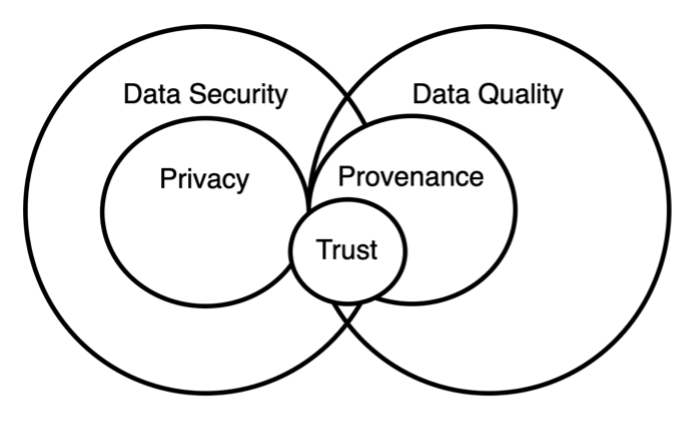
\includegraphics[]{figures/literature_review/dq_security_vs_quality.png}
    \caption{Data security vs quality}
    \label{fig:dq_security_vs_quality}
\end{figure}

\subsubsection{Data Quality Standards and Best Practice}
The ISO/DIS 8000-210 standard outlines best practices for managing sensor data quality, emphasising the importance of data accuracy, consistency, completeness, timeliness, validity, anomaly detection, and maintenance \citep{isoISODIS80002102023}. The standard offers a comprehensive framework for data quality but has limitations due to its generalised nature, complexity in implementation, and lack of flexibility that is necessary for research projects. The dimensions of data quality outlined in the standard are consistent with those identified in the literature, but the standard does not provide specific guidelines for addressing data quality issues in IoT environments. \cite{perez-castilloDataQualityBest2018a} present twenty-three best practices for data quality in IoT environments. Although the focus is largely on the implementation of the network and the data management system, some of practices are applicable to the development of a quality aware pedestrian counting platform, such as documenting quality procedures; retaining versions of input data, workflows, programs, and models used (data provenance); and performing slope and persistence checks.

\subsection{Data Quality Assessment} \label{ssec:data_quality_assessment}
\cite{immonenEvaluatingQualitySocial2015} make a useful distinction between quality assessment and quality evaluation.

\begin{itemize}
    \item \textit{Quality assessment:} assessing of the quality of raw data as  such, without considering the context or the intended use of data.
    \item \textit{Quality evaluation:} evaluating the quality of information, considering the context and the intended use of information.
\end{itemize}

This research project will mainly focus on quality assessment as the first step in the data quality management process. The dimensions of data quality identified in the previous section will be used as a foundation for assessing the quality of pedestrian data.

\subsubsection{Data Quality Assessment Methodologies}
DQ assessment is the first step in building an automated DQ pipeline. \cite{batiniMethodologiesDataQuality2009} recognise that there are many methodologies to carry out such an assessment, but identify three common phases (figure \ref{fig:dp_methodology_stages}). The first involves collecting contextual information about organisational processes, management procedures etc. The second involves measuring the value of a set of data quality dimensions and assessing the measurements against reference values. The final step concerns the selection of steps, strategies and techniques for reaching new DQ targets. As stated above, the methods investigated in this research focus mostly on the second stage, assessment and measurement of DQ.

\begin{figure}[ht]
    \centering
    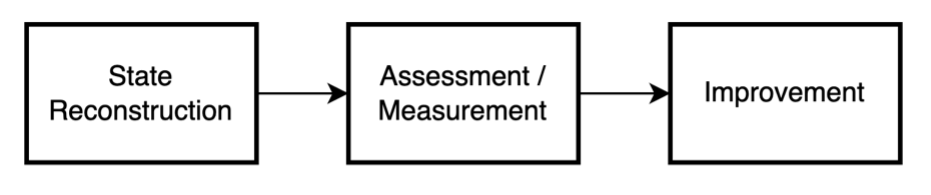
\includegraphics[]{figures/literature_review/dq_methodology_stages.png}
    \caption{General stages of DQ methodology \citep{batiniMethodologiesDataQuality2009}}
    \label{fig:dp_methodology_stages}
\end{figure}

\subsubsection{Event Detection}
Assessing data quality in WSN (time-series data) is heavily embedded in event detection. Quantifying many of the dimensions mentioned above first require understanding the ‘normal behaviour of the data’. Events are occurrences or patterns in the data that are of significant interest or importance within a specific domain or application context \citep{benabbasContextawareOutlierDetection2023}. Event detection and data quality are closely linked \citep{kumarSurveyEventDetection2023}, because all data quality issues are 'events' (patterns in the data that are of significant interest). The following sub-dimensions of data quality would need to be assessed through event detection methods when applied to real-time WSN data:

\begin{itemize}
    \item \textbf{Accuracy}: identifying data points that deviate significantly from the true or expected values, indicating potential accuracy issues.
    \item \textbf{Completeness}: detecting missing or incomplete data events, (simple) event detection techniques can assess the completeness of the incoming data.
    \item \textbf{Consistency}: identify inconsistencies and contradictions in the data by comparing data points across different sources or time periods.
    \item \textbf{Timeliness}: detecting events related to data delays, staleness, or latency can help assess the timeliness of the data.
    \item \textbf{Validity}: detection techniques can identify data points that violate predefined rules, constraints, or formats, indicating validity issues.
\end{itemize}

There are multiple approaches to event detection presented in the scientific literature. Broadly speaking, these are, rule-based methods, machine learning-based methods, deep learning-based methods, statistical and probabilistic methods, and hybrid methods \cite{kumarSurveyEventDetection2023}. Table \ref{table:event_detection_methods} gives a breakdown of what each of these methods entail.

% tables/literature_review/event_detection_methods.tex
\begin{table}[H]
    \centering
    \scriptsize % Reduce font size
    \begin{tabular}{|R{2cm}|R{6cm}|R{6cm}|}
        \hline
        \textbf{Method}               & \textbf{Examples}                                                                                       & \textbf{Description}                                                                                                        \\ \hline
        Rule-based                    & Threshold-based detection, finite state machines, and expert systems.                                   & Simple to implement but may struggle with complex event patterns and adaptability.                                          \\ \hline
        Machine learning              & Supervised learning: decision trees, support vector machines, naive Bayes, etc.

        Unsupervised learning: clustering, anomaly detection, etc.
                                      & Can adapt to complex event patterns but require sufficient labelled data for training.                                                                                                                                                \\ \hline
        Deep learning                 & Convolutional neural networks (CNNs), recurrent neural networks (RNNs), Graph neural networks (GNNs).   & Can handle high-dimensional and unstructured data but require large amounts of training data and computational resources.   \\ \hline
        Statistical and probabilistic & Hidden Markov models (HMMs), Bayesian networks, and Gaussian mixture models (GMMs).                     & Can capture the uncertainties and dependencies in event occurrences but may require prior knowledge of event distributions. \\ \hline
        Hybrid                        & Combining rule-based and machine learning methods or integrating deep learning with statistical models. & Can provide more robust and accurate event detection but may increase the complexity of the system.                         \\ \hline
    \end{tabular}
    \caption{Event detection methods for data quality}
    \label{table:event_detection_methods}
\end{table}

In the space of all domains and application contexts, every data point could, in theory, be considered an event. For the purpose of this research, the term \textit{event of interest} means a domain and application has been applied and therefore it can be considered a collapsed point appearing somewhere on Figure \ref{fig:theoretical_event_terminology}, it could be either a novelty or an anomaly, a sub-category of one or both, or neither. Figure \ref{fig:theoretical_event_terminology} is based on a number of research papers that seek to categorise types of events \citep{chandolaAnomalyDetectionSurvey2009,pimentelReviewNoveltyDetection2014,ahmadUnsupervisedRealtimeAnomaly2017,aminikhanghahiSurveyMethodsTime2017}. A brief summary of these categories is as follows:

\begin{itemize}
    \item Event - generally refers to some occurrence of interest in the system being monitored. Unusual or rare events can be considered anomalies or novelties.
    \item Anomalies - data points or patterns that deviate from the expected or normal behaviour of the system. They are often considered "abnormal" or "unusual" in the context of the system's typical operation. Anomalies can be caused by errors, faults, or malicious activities in the system. The key characteristic of an anomaly is that it deviates from the expected behaviour, regardless of whether it has been observed before.
    \item Novelty – data points or patterns that are new or previously unseen in the context of the system's operation. They represent a new behaviour or state of the system that has not been observed in the training data or during the system's normal operation. Novelties may or may not be anomalous. A novelty could represent a new normal behaviour (e.g., due to a system update or change in environment) or a new type of anomaly. The key characteristic of a novelty is its newness or previously unseen nature, regardless of whether it is normal or abnormal.
    \item Outlier - a data sequence, sub-sequence or point that lies far from the rest of the data based on some measure of distance.
    \item Discord - refers to the most unusual subsequence or sub-series within a time series.
    \item Change-point - a point in time where the behaviour of the system being monitored changes abruptly.
    \item Drift - Drift or concept drift refers to a gradual change in the behaviour of the system over time.
\end{itemize}

\begin{figure}[ht]
    \centering
    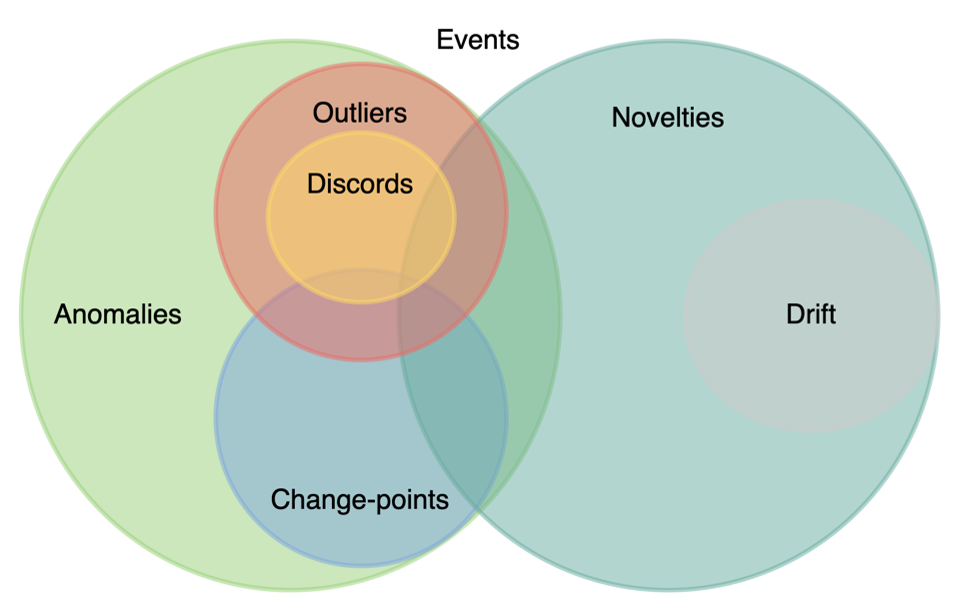
\includegraphics{figures/literature_review/theoretical_event_terminology.png}
    \caption{Theoretical event terminology}
    \label{fig:theoretical_event_terminology}
\end{figure}

These distinctions are useful because when event detection is carried out, it is often specifically outliers, discords, change-points, or drift that being directly measured though a chosen method. Once measured, these events will then be classified as either anomalies, novelties, or anomalous novelties to inform decision making \citep{abualsheikhMarkovDecisionProcesses2015}. For example, a detected anomaly, once verified as reliable, might trigger a physical response---in the context of pedestrian data this might mean dispatching an emergency services unit for crowd control. A novelty, on the other hand, might trigger the retraining of AI models as this could indicate that the factors driving pedestrian behaviour have drifted. A recent example of this is the change in pedestrian behaviour as a result of the COVID-19 pandemic \citep{chenEstimatingVehiclePedestrian2021}. As pointed out by \cite{carrenoAnalyzingRareEvent2020}, a novel anomaly would be difficult to classify autonomously as they would not be present in any training data but trigger an alert for manual analysis or model retraining.


Having identified the dimensions critical to assessing data quality in sensor data, and establishing the different groups of methods that can be applied to the problem of assessing data quality through measurement, we can begin to look at what an integrated data quality management platform for pedestrian data might look like. Three themes will be investigated in the following sections, each of these forms a process in the data management feedback loop \citep{immonenEvaluatingQualitySocial2015,ehrlingerAutomatedDataQuality2017}. These are: detection and monitoring \citep{woodallDataQualityAssessment2013,ehrlingerAutomatedDataQuality2017}; management and improvement \citep{khatriDesigningDataGovernance2010, batiniDataInformationQuality2016}; and prediction and proactive approaches \citep{liDataQualityObservation2012,ardagnaContextawareDataQuality2018}.

\begin{figure}[h]
    \centering
    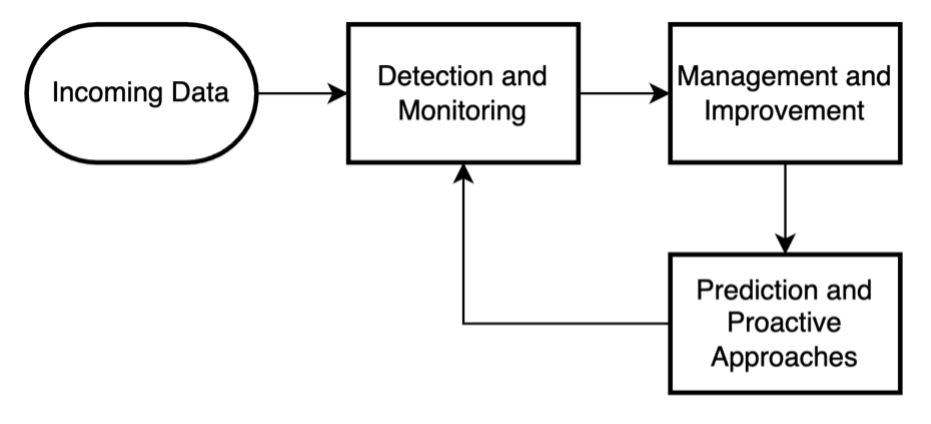
\includegraphics[]{figures/literature_review/dq_feedback_loop.png}
    \caption{Data quality feedback loop}
    \label{fig:dq_feedback_loop}
\end{figure}

\subsection{Data Quality Detection and Monitoring}\label{ssec:data_quality_detection}

This research is primarily interested in anomaly detection (defined in figure \ref{fig:theoretical_event_terminology}) which forms a binary classification problem with imbalanced classes---the objective is to categorise each instance in a dataset as belonging to one of two
possible classes: ‘‘normal’’ or ‘‘anomalous’’---shown in figure \ref{fig:outlier_decision_making}---\citep{gorsheninMobileNetworkTraffic2024}.

{\color{secondary-text-color} \textit{NOTE: Monitoring is the continuous observation and collection of data, while detection is the process of identifying specific events, anomalies, or patterns of interest within that monitored data. Monitoring provides visibility and context, while detection pinpoints specific occurrences or conditions that require attention or action \citep{tuychievComprehensiveIntroductionAnomaly2023}.}}

\subsubsection{Monitoring Methods}
There are a number of DQ dimensions that can be calculated without the need for a complicated model. \cite{fizzaAgeDataAware2022} develops a model for assessing age of data using parking sensors as a case study. The model uses a time-based calculation with spatial clustering. The authors used a heuristic approach to determine the confidence level in the state of the sensor based on the age of the data.

\begin{equation*}\label{eq:confidence_heuristic}
    Confidence = 1 - \frac{{{\text{ }}avg.Age{\text{ }}of{\text{ }}the{\text{ }}cluster{\text{ }}}}{{{\text{ }}max.Age{\text{ }}}}\tag{6}
\end{equation*}

The authors showed that this simple method could enable both better parking recommendations and highlight issues with sensor connectivity.

\subsubsection{Pattern-Based Detection Methods}
Pattern-based detection methods refer to techniques used in anomaly detection to identify specific patterns within data that correspond to known behaviours, signatures, or anomalies. These methods rely on predefined rules or models that describe what constitutes a normal or abnormal pattern in the dataset \citep{caiMinimalRarePatternBased2023}.

Detection requires identifying events. There are a number of approaches to this in the literature following the approaches shown in table \ref{table:event_detection_methods} above. \cite{kleinRepresentingDataQuality2009} present a methodology based on sliding windows that follow a rule-based approach utilising fast Fourier transform (FFT) to assess signal behaviour (table \ref{table:interest_indicators}). One downside to this approach is that FFT requires complete time-series data windows to work, meaning some sort of missing data imputation would need to be carried out first. However, there are methods like the Lomb-Scargle periodogram, that can create similar outputs to FFT on incomplete data \citep{vanderplasUnderstandingLombScargle2018}.

% tables/literature_review/interest_indicators.tex
\begin{table}[H]
    \centering
    \scriptsize % Make the text smaller
    \begin{tabular}{|M{2cm}|M{2cm}|M{8cm}|}
        \hline
        \textbf{Example function}   & \textbf{Interest indicator}     & \textbf{DQ control operator pattern}                                              \\ \hline
        \textbf{$current\_value()$} & Extraordinary value ranges      & 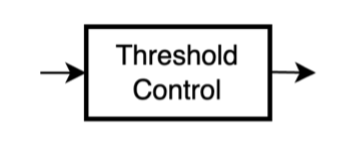
\includegraphics[scale=0.75]{figures/literature_review/interest_indicators_1.png} \\ \hline
        \textbf{$sliding\_slope()$} & Extraordinary value alterations & 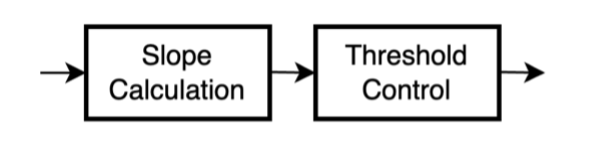
\includegraphics[scale=0.75]{figures/literature_review/interest_indicators_2.png} \\ \hline
        \textbf{$fft\_slope()$}     & Changing periodicity            & 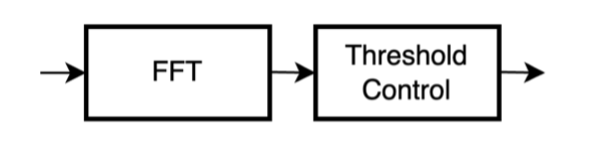
\includegraphics[scale=0.75]{figures/literature_review/interest_indicators_3.png} \\ \hline
        \textbf{$fft()$}            & Unsteadiness                    & 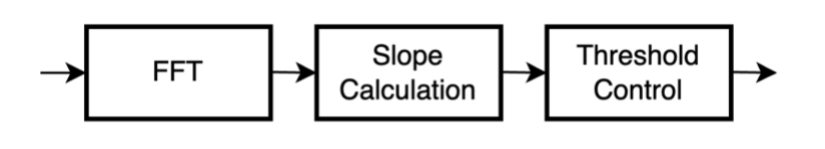
\includegraphics[scale=0.75]{figures/literature_review/interest_indicators_4.png} \\ \hline
    \end{tabular}
    \caption{Interest indicators and operators (Klein and Lehner 2009)}
    \label{table:interest_indicators}
\end{table}

\subsubsection{Real-Time Monitoring and Event-Driven Architecture}
System architecture is an important component in detection and monitoring as it requires a number of different processes running together. \cite{mehmoodNovelEdgeArchitecture2024} develop a portable hybrid architecture for smart cities based on device edge and cloud computing. The hybrid system combines LSTMs, PageHinkley test, adaptive windowing, and Kolmogorov-Smirnov windowing. \cite{simsekDeepFogAQFogassistedDecentralized2024} integrate Transformers, CNN-LSTM, GRU, and RFR models into their hybrid deep-learning detection system that uses fog computing, complex event processing, and virtualisation to do event detection. Whilst these systems are not directly applicable to the research, they provide a good foundation for understanding the architecture of a real-time monitoring system.

\subsubsection{Outlier Detection}
If a sensor frequently produces outliers, it may indicate issues with sensor calibration, environmental conditions, or measurement techniques. By detecting and analysing patterns in outliers, we can assess the reliability of the sensor data and make adjustments to improve certainty. Common outlier detection methods from literature include:

\begin{itemize}
    \item Statistical methods: These methods assume that the data follows a particular distribution (e.g., Gaussian) and identify outliers based on statistical measures, such as mean, median, standard deviation, or interquartile range \citep{iglewiczVolume16How1993,aggarwalOutlierEnsembles2017}.
    \item Distance-based methods: These methods identify outliers based on their distance from other data points. Examples include k-nearest neighbours (k-NN) and Local Outlier Factor (LOF) \citep{ramaswamyEfficientAlgorithmsMining2000,breunigLOFIdentifyingDensitybased2000}
    \item Density-based methods: These methods detect outliers based on the density of data points in their neighbourhood. Examples include DBSCAN and OPTICS \citep{esterDensityBasedAlgorithmDiscovering1996, ankerstOPTICSOrderingPoints1999}.
    \item Machine learning methods: These methods employ machine learning algorithms, such as support vector machines (SVM) or deep learning, to learn patterns in the data and identify outliers based on their deviations from these patterns \citep{blazquez-garciaReviewOutlierAnomaly2021}.
\end{itemize}

\cite{shuklaScalableRobustOutlier2020} propose a scalable outlier detector using hierarchical clustering and LSTM neural networks, demonstrating high accuracy and outlier sensitivity tuning capabilities. \cite{nguyenForecastingAnomalyDetection2021} combine LSTM auto-encoders with one-class SVM for anomaly detection, achieving promising results on benchmark datasets and fashion retail data. There are a number of classifying types of outlier for WSN, \cite{zhangOutlierDetectionTechniques2010} divide these into events detection, malicious attack detection, and noise and error detection (Figure \ref{fig:outlier_detection_categories}).

\begin{figure}[h]
    \centering
    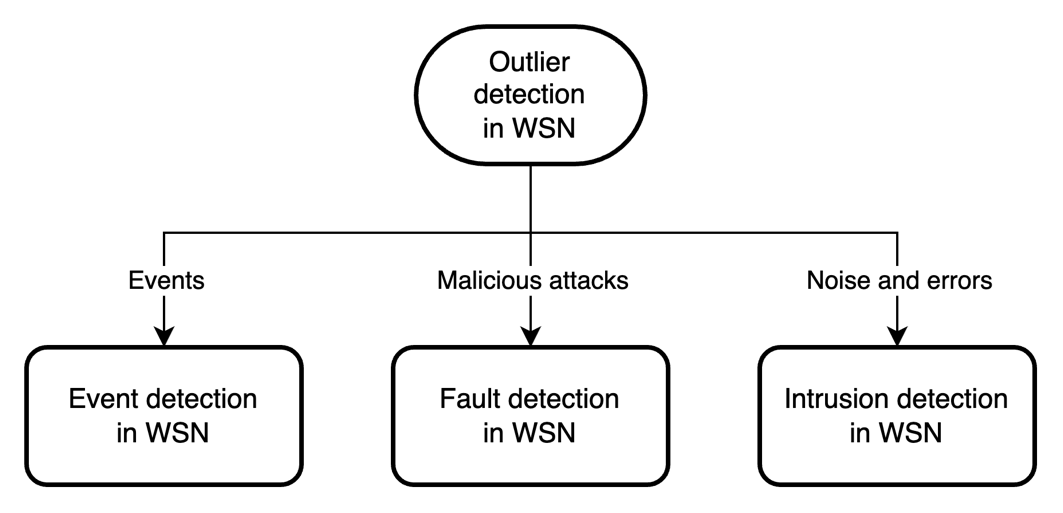
\includegraphics{figures/literature_review/outlier_detection_categories.png}
    \caption{Outlier detection categories based on \cite{zhangOutlierDetectionTechniques2010}
    }
    \label{fig:outlier_detection_categories}
\end{figure}

\cite{dingLocalizedFaulttolerantEvent2005} stress the importance of identifying the boundaries of important events in wireless sensor networks rather than just the regions where these events occur. This focus is due to the unreliability of sensor measurements. They explain the main differences between detecting important events and outlier detection. These differences include:

\begin{itemize}
    \item Prior knowledge of trigger conditions: Knowing what triggers an event is crucial for detecting important events, while outlier detection does not require this knowledge.
    \item Goals: Event detection aims to specify events of interest, whereas outlier detection focuses on identifying unusual readings.
    \item Misclassification: In outlier detection, it’s important to avoid classifying normal data as outliers. In event detection, the goal is to prevent incorrect data from affecting the reliability of detecting important events.
\end{itemize}

Despite these differences, both techniques use the spatial and temporal correlations among sensor data from nearby nodes to distinguish between actual events and errors. Event measurements are usually spatially related, while noisy measurements and sensor faults are not \cite{tehSensorDataQuality2020}. Although outlier detection techniques might work for event detection, they are not commonly used in this field because not all outliers need to be identified for event detection purposes. In the context of figure \ref{fig:outlier_detection_categories}, an event of interest is one that has led to erroneous data and triggers data cleaning.

\begin{figure}[h]
    \centering
    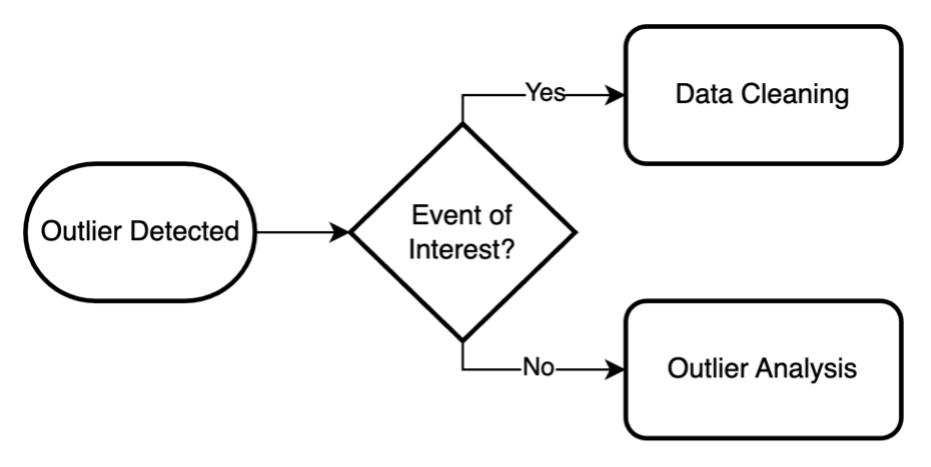
\includegraphics{figures/literature_review/outlier_decision_making.png}
    \caption{Decision making as a result of outlier analysis based on \cite{blazquez-garciaReviewOutlierAnomaly2021}}
    \label{fig:outlier_decision_making}
\end{figure}

\subsubsection{Abnormal Node Detection in WSN}
Abnormal node detection in wireless sensor networks refers to the process of identifying nodes that exhibit unusual or anomalous behaviour compared to the expected normal behaviour of the nodes in the network \citep{liNearestNeighborImputation2014}. In the context of urban mobility data such as pedestrian counts, abnormal mode detection is needed to differentiate between real events such as overcrowding of a metro station and erroneous events arising from detection faults.

\cite{chenFaultDetectionMethod2021} take a traditional approach using multi-step methodology using spatio-temporal correlation to detect abnormal nodes. They first calculate the offset between a historic window and the current window to evaluate temporal consistency. They then use a nearest neighbour algorithm cluster the data. They combine the result of spatial and temporal offsets and repeat for all nodes in the network. Whilst the results show that this method outperforms others, the authors acknowledge that this method is computationally expensive and may not be suitable for large networks or real-time applications.

\cite{zhangNovelAnomalyDetection2022} propose an anomaly detection method for multimodal WSN data flow via a dynamic graph neural network. The authors inject four types of anomalies into the testing data:

\begin{itemize}
    \item Anomaly type 1 simulates slow mode changes in the environment detected by a node that deviates from its conventional state (e.g. the observed value of the gas content of a sensor node gradually increases due to the leakage of toxic gas in the chemical plant).
    \item Anomaly type 2 simulates fast mode changes in the environment detected by a node (e.g. the temperature observation of a sensor node rises rapidly in a short period of time due to a fire).
    \item Anomaly type 3 simulates extreme changes in the external environment detected by a node (e.g. the sudden invasion of high-temperature sources leads to sudden changes in the temperature observations).
    \item Anomaly type 4 simulates the failure of a sensor node due to external interference, and the observed value of the mode becomes 0.
\end{itemize}

The authors use a GRU as it is less computationally expensive that an LSTM which shows promising results for real-time applications.

    {\color{secondary-text-color} \textit{NOTE: In this experiment the GRU performed best a window length of 60 data points and an output layer size of 32. The authors also found that using min-max normalisation compared to z-score normalisation resulted in high misjudgement rate.}}

\subsection{Data Quality Management and Improvement}\label{ssec:data_quality_management}

Although data quality improvement is beyond the scope of this research, it is important to be cognisant of these methods to  inform development decisions for the quality-aware system. There a number of different methods for achieving this.

\subsubsection{Correcting Errors}

\cite{tehSensorDataQuality2020} identify two categories of error correcting methods in WSN data, \textit{missing data imputation} which attempts to correct estimate sensor measurement values that are missing and \textit {de-noising} which aims to remove the noise associated with the measurement signal. The authors references a number of different methods for each of these categories, including: association rule mining \citep{gruenwaldUsingDataMining2007}, clustering \citep{tangHybridApproachIntegrate2015} where the authors use a hybrid model for for missing traffic volume estimation, k-nearest neighbour \citep{liNearestNeighborImputation2014}, and single-value decomposition \citep{xuInterpolatingMissingValues2017} which the authors demonstrate on real-world air quality datasets.

\subsubsection{Data Management Platform Architecture: Case Studies}

Management frameworks for IoT/WSN follow a few main themes: edge computing; data integration techniques; cloud computing; and data analytics. \cite{badidiBuildingDataPipeline2018} identify key features an urban data stream management and processing pipeline as: facilitating real-time event detection; notification of alerts; mining the opinions of citizens regarding the governance of their city; and building monitoring dashboards. The authors implement a prototype of the using the Kafka messaging platform. Whilst there are a number of systems that have been developed for managing data streams, there are few that focus on data quality management that have been fully implemented. \cite{ehrlingerDaQLMonitorData2019} present a data quality management methodology that uses machine learning algorithms to detect and correct data quality issues in real-time for industrial IoT applications, which is the closest to a functioning management system for WSN data in the literature.

\subsection{Data Quality Reliability and Proactive Approaches} \label{ssec:data_quality_prediction}

This sections looks at how future data quality can be improved through predictive modelling for sensor optimisation and proactive data quality management strategies. This includes understanding optimal sensor placement \citep{kimOptimizationNumberWireless2024} and improving checks on incoming data \citep{mohammadiSmartCityDigital2017}. This section differs from the previous, in that rather than trying to detect and correct errors, it is concerned with optimising the WSN to prevent errors from occurring in the first place.

\subsubsection{Fault Tolerance}

Fault tolerance in wireless sensor networks (WSNs) refers to the network’s ability to continue functioning correctly even in the presence of failures or errors within some of its components. This includes the capability to handle node failures, communication errors, or environmental disruptions without significant loss of data or performance \citep{guravaiahDataCollectionProtocols2020}. There are a number of methods involved in building fault tolerant WSNs, including: redundancy, error detection and correction, and self-healing mechanisms \citep{guravaiahDataCollectionProtocols2020}. \cite{elkhediriWirelessSensorNetworks2022} present a comprehensive review of fault tolerance in WSNs, highlighting the importance of clustering protocols to ensure that data is not lost in the event of a node failure.

\subsubsection{Preventative Measures}

\cite{chengDataQualityAnalysis2018} explore the relationship between different data quality evaluation indicators to carry out a variety of data cleaning strategies. The results showed that the proposed strategies can improve data availability and reduce cleaning costs (computational overhead and time) for errors such as data loss, sample jitter, and gross error. The order of cleaning strategies was found to be important--starting with completeness cleaning (to repair lost data) followed by time-related cleaning (to eliminate sampling jitter) and finally correctness cleaning (to correct abnormal data) is found to be the most effective sequence. \cite{kleinRepresentingDataQuality2009} suggest a strategy of carefully surveying data quality restrictions and propagating quality information through data processing pipelines. They introduce jumping data quality windows to reduce data overhead and propose methods for data quality recording and storage. However, the experiments were tested on synthetic data and the authors acknowledge that further research is needed to validate the results on real-time, real-world data.

\subsection{Challenges and Future Directions} \label{ssec:challenges_and_future_directions}

\subsubsection{Scalability}
Scalability is a critical consideration in the development of data quality management systems for wireless sensor networks (WSNs), especially in the context of pedestrian monitoring in smart cities. As WSNs grow in size and complexity, several challenges arise that must be addressed to ensure effective and efficient data collection, processing, and analysis. Increasing the number of sensor nodes to cover larger urban areas can lead to higher data traffic, causing congestion and potential data loss. Dense networks also pose challenges in terms of interference and overlapping signals, which can degrade data quality \cite{akyildizWirelessSensorNetworks2002}. The volume of data generated by a large number of sensors means automated management processes are required, necessitating significant computational resources and efficient algorithms for real-time processing and storage \cite{gubbiInternetThingsIoT2013}.

Ensuring data quality across a large and diverse network is complex, with issues such as data inconsistency, missing data, and noise becoming more pronounced as the network scales \cite{karkouchDataQualityInternet2016}. Real-time data processing is essential for applications like pedestrian monitoring, where timely information is critical, increasing the demand for real-time processing capabilities \cite{ahmadUnsupervisedRealtimeAnomaly2017}. As networks scale, the likelihood of node failures and communication errors increases, making fault tolerance and reliable data transmission more challenging \cite{younisStrategiesTechniquesNode2008}. Addressing these scalability challenges requires a combination of advanced data management techniques, energy-efficient protocols, and robust fault-tolerance strategies to ensure that WSNs can provide reliable and high-quality data for pedestrian monitoring in smart cities.

\subsubsection{Integration}
With the proliferation of platforms such as the one proposed here it becomes increasingly important for them to be able to integrate with other systems. This requires centralised governance and standardisation. This exists at a high level with the Gemini principles \citep{waltersGeminiPrinciples2019} and the National Digital Twin project \citep{NationalDigitalTwin2024} which deal with ethics and governance and are primarily driven by purpose (what do we want from digital twins). A more low-level data-focussed standards can be found in the Open Geospatial Consortium's CityGML and Moving Features standards \citep{OGCMovingFeatures2024,CityGML2024}, and the INSPIRE directive \citep{INSPIREKnowledgeBase2024} from the European Commission are more data-focussed and policy focussed respectively. These standards are important for ensuring interoperability and scalability in smart city applications, and are essential for the development of a robust and scalable system for managing pedestrian data quality.

\subsection{Summary}

This literature review has explored the critical aspects of data quality in wireless sensor networks (WSNs) with a focus on pedestrian monitoring. Key dimensions such as accuracy, completeness, consistency, timeliness, and validity have been examined, highlighting the importance of maintaining high data quality for reliable pedestrian data.

Methodologies for data quality assessment, including statistical measures, machine learning approaches, and event detection techniques, have been reviewed. These methodologies are essential for real-time detection and monitoring of data anomalies, ensuring the reliability of pedestrian counts. The review also covered strategies for managing and improving data quality, such as automated imputation for missing data and denoising techniques, which are crucial for maintaining data integrity. Enhancements in WSN architecture aimed at improving data quality from the source were discussed, providing insights into building a scalable pedestrian data quality management system. Challenges and future directions emphasise the need for centralised governance and standardisation when building such platforms, ensuring interoperability and scalability in smart city applications. This research contributes to the development of a robust and scalable system for managing pedestrian data quality, facilitating more accurate and reliable urban mobility monitoring.

In summary, maintaining high data quality in WSNs for pedestrian monitoring requires a comprehensive approach, integrating advanced data quality assessment methodologies, real-time monitoring, and proactive management. This ongoing research aims to address current challenges and support the creation of effective, scalable data quality management systems for smart cities.